% !TeX program = pdflatex
\documentclass[runningheads]{llncs}

% --- Packages ---
\usepackage[T1]{fontenc}
\usepackage[utf8]{inputenc}
\usepackage{graphicx}
\usepackage{hyperref}
\usepackage{booktabs}
\usepackage{csquotes}
\usepackage{amsmath}
\usepackage{enumitem}
\usepackage{xcolor}
\usepackage{caption}
\usepackage{subcaption}
\usepackage{tikz}
\usetikzlibrary{arrows.meta, positioning, calc}

% --- Metadata ---
\title{ThesisFlow: Plataforma Web para la Gestión y Visualización de Trabajos Finales en el DCIC}
\titlerunning{ThesisFlow}
\author{Ignacio Joaqu\'in Dotta}
\authorrunning{I. J. Dotta}
\institute{Departamento de Ciencias e Ingenier\'ia de la Computaci\'on (DCIC)\\
Universidad Nacional del Sur, Argentina\\
Directores: Dr. Martín Larrea y Dra. María Luján Ganuza\\
Codirector: Lic. Diego Sebastian Orbe Leiva\\
\email{\{ignacio.dotta, mlg, mll, diego.orbe\}@cs.uns.edu.ar}}

\begin{document}
\maketitle

% --- Abstract ---
\begin{abstract}
Este trabajo presenta \emph{ThesisFlow}, una plataforma web que centraliza la gestión y visualización de Trabajos Finales y Tesis de Grado del DCIC. El sistema integra en una única solución los flujos administrativos de carga y curado de información, un módulo de autogestión para docentes y un portal público de analíticas interactivas. Se describen la motivación y el contexto institucional, la exploración de soluciones y alternativas, los objetivos del proyecto y los aspectos centrales de la implementación a nivel de arquitectura, modelo de datos e interfaces. Finalmente, se discuten usos concretos de la aplicación, conclusiones sobre su impacto y líneas de trabajo futuro.
\keywords{Sistemas de información académica \and Visualización de datos \and Ingeniería de software \and Aplicaciones web}
\end{abstract}

% --- 1. Motivación ---
\section{Motivación}

La gestión de Trabajos Finales y Tesis de Grado en el Departamento de Ciencias e Ingeniería de la Computación (DCIC) involucra a secretaría, docentes, estudiantes y autoridades. Históricamente, la información asociada a estos proyectos se distribuyó en planillas, documentos aislados y actas del Consejo Departamental, lo que dificulta:

\begin{itemize}
  \item la trazabilidad del ciclo de vida de cada trabajo;
  \item el análisis de tendencias temáticas y líneas de dirección;
  \item la obtención de estadísticas confiables para la planificación académica;
  \item la transparencia institucional respecto de la producción del departamento.
\end{itemize}

\subsection*{Estado del arte}

Tradicionalmente, al preparar la producción académica anual se revisan manualmente las actas aprobadas durante el período correspondiente, obteniendo principalmente conteos agregados de Trabajos Finales. En años recientes se comenzó a recopilar información más detallada (título, fechas, docentes, temática, alumnos), pero sin un sistema que permita explotarla de manera estructurada ni ofrecer vistas unificadas a los distintos actores.

\subsection*{Perspectiva de los estudiantes}

Desde la óptica de los alumnos, el inicio del Trabajo Final suele estar acompañado de incertidumbre. Son frecuentes situaciones como:

\begin{itemize}
  \item no tener claro qué tipo de producto o alcance se espera de un Trabajo Final;
  \item contar con una idea preliminar pero no saber si es viable o qué docente podría dirigirla;
  \item desconocer qué temas se han trabajado recientemente en el departamento.
\end{itemize}

Una plataforma integral que brinde acceso a proyectos históricos, sus temas y docentes asociados permite:

\begin{itemize}
  \item explorar Trabajos Finales previos y su documentación para inspirarse;
  \item identificar tendencias temáticas a lo largo del tiempo;
  \item partir de un tema de interés y localizar qué docentes trabajan en esa área;
  \item partir de un docente y explorar los temas en los que ha dirigido trabajos.
\end{itemize}

En este contexto, \emph{ThesisFlow} surge como una herramienta para unificar la gestión, facilitar el acceso a la información y habilitar analíticas que apoyen la toma de decisiones de estudiantes y autoridades.

% --- 2. Exploración de soluciones ---
\section{Exploración de soluciones}

Previo al diseño de la plataforma se revisaron soluciones existentes vinculadas a la gestión y difusión de Trabajos Finales y Tesis. Entre ellas se consideraron:

\begin{itemize}
  \item Repositorio UBA: \url{https://repositoriouba.sisbi.uba.ar/gsdl/cgi-bin/library.cgi}
  \item Repositorio Digital de la UNS: \url{https://repositoriodigital.uns.edu.ar/}
\end{itemize}

Estos repositorios permiten almacenar y consultar trabajos completos, junto con metadatos básicos sobre autores, directores y fecha. Sin embargo:

\begin{itemize}
  \item no incorporan flujos administrativos específicos del DCIC (por ejemplo, carga desde actas del Consejo);
  \item no brindan analíticas interactivas sobre temas, carreras o redes de colaboración;
  \item no ofrecen vistas diferenciadas para secretaría, docentes y estudiantes.
\end{itemize}

También se analizaron sistemas de gestión académica y plataformas de e-learning con módulos de Trabajos Finales. En general, se observó que cubren parcialmente el problema, con escasa capacidad de adaptación al dominio local y limitadas herramientas de visualización de datos.

% --- 3. Alternativas ---
\section{Alternativas}

A partir de la exploración previa se identificaron tres alternativas principales:

\subsection*{1. Mantener el esquema actual}

La primera opción consistía en continuar utilizando planillas compartidas y documentos dispersos. Esta alternativa se descartó debido a:

\begin{itemize}
  \item dificultades para garantizar integridad y uniformidad de los datos;
  \item escasa capacidad de visualización avanzada y analíticas complejas;
  \item poca escalabilidad a medida que crece el volumen de Trabajos Finales;
  \item limitaciones para extender funcionalidades o incorporar nuevos actores.
\end{itemize}

\subsection*{2. Adoptar un sistema externo}

La segunda alternativa era adaptar un sistema existente (repositorio institucional, sistema académico o plataforma de terceros). Si bien podría reducir esfuerzo inicial, presenta desventajas:

\begin{itemize}
  \item menor flexibilidad para adaptar el modelo de datos al DCIC;
  \item dependencia de un proveedor externo para la evolución del sistema;
  \item capacidades analíticas y de personalización acotadas.
\end{itemize}

\subsection*{3. Desarrollar un sistema propio}

La tercera opción, finalmente adoptada, es desarrollar una solución propia, modular y extensible. Esta alternativa supone un mayor esfuerzo inicial, pero ofrece:

\begin{itemize}
  \item control total sobre el modelo de datos y las reglas de negocio;
  \item optimización específica para consultas y analíticas relevantes;
  \item un diseño preparado para extenderse a nuevas carreras o módulos (por ejemplo, posgrado);
  \item posibilidad de incorporar integración progresiva con otros sistemas institucionales.
\end{itemize}

% --- 4. Especificación de objetivos ---
\section{Especificación de objetivos}

\subsection{Objetivo general}

Diseñar e implementar una plataforma web integral para la gestión, el seguimiento y la visualización de Trabajos Finales y Tesis de Grado del DCIC, que sirva como fuente confiable de información para secretaría, docentes y comunidad académica.

\subsection{Objetivos específicos}

\begin{itemize}
  \item Centralizar la información de Trabajos Finales en una base de datos estructurada y consistente.
  \item Proveer interfaces diferenciadas para secretaría, docentes y público general.
  \item Ofrecer analíticas interactivas sobre la producción del departamento.
  \item Incorporar mecanismos de autenticación y control de acceso acordes a cada perfil.
  \item Facilitar tareas de respaldo, restauración y auditoría de datos.
\end{itemize}

% --- 5. Implementación ---
\section{Implementación}

\subsection{Arquitectura general}

La arquitectura de \emph{ThesisFlow} adopta una estructura de tres capas: frontend, backend y base de datos. La Figura~\ref{fig:architecture} ilustra los componentes principales y sus interacciones.

\begin{figure}[h]
\centering
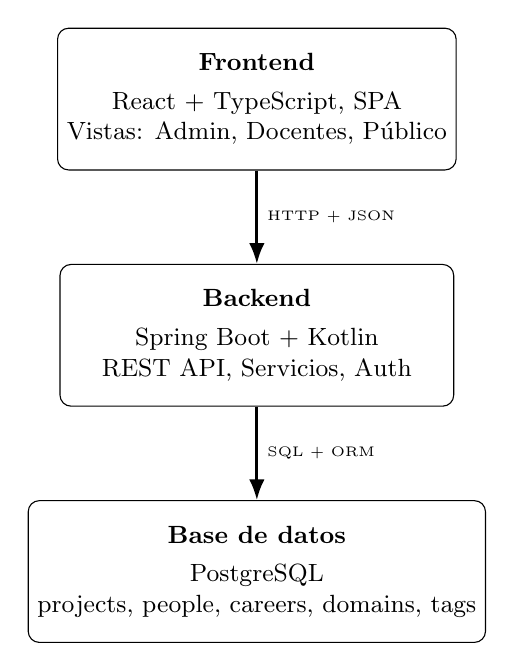
\begin{tikzpicture}[
  box/.style={
    rectangle,
    draw,
    rounded corners,
    align=center,
    minimum width=5cm,
    minimum height=1.8cm,
    font=\small
  },
  arrow/.style={-Latex, line width=1pt}
]

% Frontend (top)
\node[box] (fe) at (0, 6) {%
  \textbf{Frontend}\\[3pt]
  React + TypeScript, SPA\\
  Vistas: Admin, Docentes, Público
};

% Backend (middle)
\node[box] (be) at (0, 3) {%
  \textbf{Backend}\\[3pt]
  Spring Boot + Kotlin\\
  REST API, Servicios, Auth
};

% Base de datos (bottom)
\node[box] (db) at (0, 0) {%
  \textbf{Base de datos}\\[3pt]
  PostgreSQL\\
  projects, people, careers, domains, tags
};

% Relaciones entre capas
\draw[arrow] (fe) -- node[right, font=\tiny]{HTTP + JSON} (be);
\draw[arrow] (be) -- node[right, font=\tiny]{SQL + ORM} (db);

\end{tikzpicture}
\caption{Arquitectura general de \emph{ThesisFlow}: tres capas principales y sus responsabilidades.}
\label{fig:architecture}
\end{figure}

El backend expone endpoints REST para operaciones administrativas, vistas públicas y analíticas. Los servicios encapsulan la lógica de negocio (gestión de proyectos, personas, carreras, importación y respaldos). El frontend, implementado como SPA, organiza vistas por rol y utiliza componentes reutilizables para formularios, tablas y dashboards.

\subsection{Modelo de datos y servicios}

El modelo de datos incluye entidades como \texttt{Project}, \texttt{Person}, \texttt{Career}, \texttt{Domain} y \texttt{Tag}, junto con tablas de unión para representar relaciones muchos-a-muchos (por ejemplo, proyectos–docentes y proyectos–etiquetas). Internamente se utilizan claves enteras, mientras que hacia el exterior se exponen UUIDs para preservar estabilidad y privacidad en los identificadores.

Los servicios de negocio abstraen el acceso a datos y coordinan operaciones que involucran múltiples entidades, tales como la creación de un nuevo proyecto con sus relaciones, la importación de lotes desde archivos CSV o la construcción de agregados para analíticas.

\subsection{Decisiones de diseño y proceso de desarrollo}

El desarrollo de \emph{ThesisFlow} involucró una serie de decisiones arquitectónicas y metodológicas que respondieron tanto a los requisitos funcionales como a las necesidades operativas del DCIC. A continuación se detallan algunos de los aspectos más relevantes.

\paragraph{a) Flujo de autenticación mediante \emph{magic links}.}
Para facilitar el acceso de los docentes sin requerir usuarios y contraseñas tradicionales, se implementó un mecanismo de acceso basado en \emph{magic links}. El flujo consiste en:
\begin{itemize}
  \item El profesor solicita acceso proporcionando su correo institucional.
  \item El sistema genera un enlace único asociado a un token efímero (no JWT) y lo envía al correo correspondiente. Este correo debe coincidir con el registrado previamente por secretaría al cargar proyectos dirigidos por ese docente.
  \item Al acceder desde el enlace, el backend valida el token y emite un JWT estándar, que el frontend utiliza para autenticar las sesiones posteriores del docente.
\end{itemize}
Este mecanismo evita la gestión de contraseñas, reduce fricción para los usuarios y mantiene un esquema seguro basado en la posesión del correo institucional.

\paragraph{b) Elección de un modelo estructurado en SQL.}
Aunquue la estructura jerárquica de un Trabajo Final podría modelarse en una base NoSQL, se optó por PostgreSQL debido a:
\begin{itemize}
  \item la necesidad de garantizar consistencia y normalización de datos;
  \item la presencia de relaciones complejas entre entidades (proyectos, docentes, estudiantes, carreras, etiquetas);
  \item la importancia de realizar estadísticas precisas, agregaciones y filtros sobre datos altamente estructurados.
\end{itemize}
Un modelo NoSQL hubiera simplificado algunos aspectos del dominio, pero hubiera dificultado mantener consistencia cuando cambian datos compartidos, como la información de un docente asociado a múltiples proyectos.

\paragraph{c) Proceso de desarrollo.}
El desarrollo se organizó en etapas sucesivas:
\begin{itemize}
  \item Reuniones iniciales para análisis de requerimientos y definición del alcance general.
  \item Elaboración de un documento PRD (\emph{Product Requirements Document}) con requerimientos funcionales detallados.
  \item Priorización en tres hitos principales:
  \begin{enumerate}
    \item Modelo de datos, CRUDs administrativos y autenticación de secretaría.
    \item Acceso público, visualizaciones interactivas y motor de analíticas.
    \item Funcionalidades específicas para docentes, incluyendo vistas personalizadas y \emph{magic links}.
  \end{enumerate}
  \item Creación de prototipos de interfaz en Figma para validar flujos y orientar el diseño visual.
  \item Diseño del modelo entidad–relación (ER) y transición a la implementación incremental.
\end{itemize}

\paragraph{d) Uso experimental de herramientas de inteligencia artificial.}
Durante el desarrollo se integraron herramientas de IA generativa (Claude Haiku 4.5 y Codex/ChatGPT 5.0) para acelerar tareas repetitivas. Se observó:
\begin{itemize}
  \item Alta utilidad en generación de componentes de frontend, CRUDs, pruebas automáticas y depuración de errores típicos de librerías.
  \item Utilidad moderada en tareas de refactorización o generación de código boilerplate.
  \item Limitaciones marcadas en tareas complejas como diseño del servicio de analíticas, donde la IA tendió a producir errores conceptuales o resultados inconsistentes.
\end{itemize}
En conclusión, la IA se demostró altamente eficaz para acelerar un proyecto de escala media cuando se aplica a tareas bien definidas y supervisadas, reduciendo significativamente tiempos de desarrollo.

\subsection{Despliegue e infraestructura}

En el entorno actual, el frontend de \emph{ThesisFlow} se despliega en Vercel, que realiza el proceso de construcción utilizando la configuración de Vite.js y sirve los archivos estáticos resultantes desde su red de distribución de contenido. El backend y la base de datos PostgreSQL se alojan en Render, donde el servicio backend se construye y ejecuta a partir de un \texttt{Dockerfile}, lo que permite reproducir localmente el mismo entorno de ejecución que en producción.

Como línea de mejora, se considera deseable que a futuro la plataforma sea alojada en la infraestructura del propio DCIC, bajo un dominio institucional del tipo \texttt{*.cs.uns.edu.ar}, de modo de consolidar el control operativo, la soberanía de los datos y la integración con otros servicios de la Universidad.

\subsection{Carga inicial de datos}

La carga inicial de datos constituyó una etapa fundamental para poner en funcionamiento la plataforma con un conjunto completo y confiable de Trabajos Finales históricos. El proceso se estructuró en tres fases principales: normalización del dataset original, preparación estructurada de los archivos y carga mediante la funcionalidad de importación masiva del sistema.

\paragraph{Normalización y limpieza del dataset.}
El punto de partida fue un conjunto heterogéneo de fuentes: planillas históricas, documentos administrativos y actas del Consejo Departamental. Estos datos presentaban variaciones en nombres de docentes, formatos de fechas, diferencias tipográficas y estructuras inconsistentes.  
Para unificar estos registros, se desarrolló un script específico (documentado en el repositorio del proyecto) que:

\begin{itemize}
  \item estandarizó nombres de docentes y estudiantes mediante reglas de coincidencia aproximada y diccionarios de equivalencias;
  \item unificó formatos de fechas (aprobación, defensa, publicación);
  \item asignó carreras y dominios respetando taxonomías actuales del DCIC;
  \item detectó y resolvió duplicados mediante heurísticas basadas en título + año + docente;
  \item generó UUIDs estables para cada proyecto y persona.
\end{itemize}

Este proceso garantizó un dataset coherente y apto para ser cargado en un modelo relacional.

\paragraph{Preparación del archivo de importación.}
Una vez normalizado el dataset, el script generó un archivo CSV con columnas alineadas al modelo de datos interno: proyecto, fechas, docentes, carrera, etiquetas temáticas y dominios.  
El sistema comprueba automáticamente la validez del archivo, la consistencia de las columnas y el tipo de datos antes de continuar.

\paragraph{Importación masiva en la plataforma.}
Finalmente, la carga se realizó utilizando la funcionalidad de “Importar proyectos”, que:

\begin{itemize}
  \item procesa cada fila como una operación atómica (validación → creación del proyecto → creación de relaciones);
  \item informa errores fila por fila sin detener el proceso completo;
  \item genera un reporte detallado con estadísticas (creados, actualizados, rechazados);
  \item asegura que las entidades relacionadas (docentes, etiquetas, dominios) se creen o reutilicen según corresponda.
\end{itemize}

Gracias a este proceso, el sistema quedó poblado con la totalidad del historial disponible, permitiendo que las visualizaciones y analíticas fueran significativas desde el primer despliegue.

\subsection{Flujo de creación de proyectos}

El flujo de creación de un proyecto refleja el proceso que sigue la secretaría para registrar un Trabajo Final aprobado. La Figura~\ref{fig:sequence} muestra un diagrama de secuencia simplificado.

\begin{figure}[h]
\centering
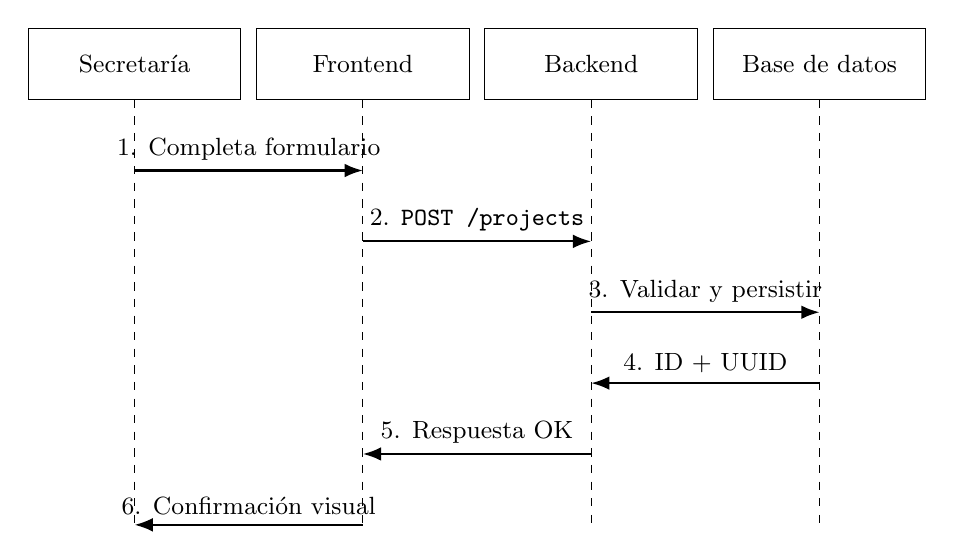
\begin{tikzpicture}[
  font=\small,
  lifeline/.style={rectangle, draw, minimum width=2.7cm, minimum height=0.9cm, align=center},
  flow/.style={-Latex, line width=0.8pt},
  x=2.9cm,
  y=1cm
]

% Lifeline headers
\node[lifeline] (admin) at (0,0) {Secretaría};
\node[lifeline] (fe) at (1,0) {Frontend};
\node[lifeline] (be) at (2,0) {Backend};
\node[lifeline] (dbs) at (3,0) {Base de datos};

% Lifeline dashed
\draw[dashed] (admin.south) -- ++(0,-5.4);
\draw[dashed] (fe.south) -- ++(0,-5.4);
\draw[dashed] (be.south) -- ++(0,-5.4);
\draw[dashed] (dbs.south) -- ++(0,-5.4);

% Messages (explicit vertical levels)
\draw[flow] ($(admin.south)+(0,-0.9)$) -- node[above]{1. Completa formulario} ($(fe.south)+(0,-0.9)$);
\draw[flow] ($(fe.south)+(0,-1.8)$) -- node[above]{2. \texttt{POST /projects}} ($(be.south)+(0,-1.8)$);
\draw[flow] ($(be.south)+(0,-2.7)$) -- node[above]{3. Validar y persistir} ($(dbs.south)+(0,-2.7)$);
\draw[flow] ($(dbs.south)+(0,-3.6)$) -- node[above]{4. ID + UUID} ($(be.south)+(0,-3.6)$);
\draw[flow] ($(be.south)+(0,-4.5)$) -- node[above]{5. Respuesta OK} ($(fe.south)+(0,-4.5)$);
\draw[flow] ($(fe.south)+(0,-5.4)$) -- node[above]{6. Confirmación visual} ($(admin.south)+(0,-5.4)$);

\end{tikzpicture}

\caption{Flujo simplificado de creación de un proyecto en \emph{ThesisFlow}.}
\label{fig:sequence}
\end{figure}

Este flujo asegura que los datos ingresados se validen en el backend, que se creen las relaciones necesarias en la base de datos y que el nuevo proyecto quede disponible inmediatamente para las interfaces de consulta y analíticas.

% --- 6. Usos de la app ---
\section{Usos de la aplicación}

\emph{ThesisFlow} se utiliza en distintos escenarios por actores con necesidades diversas:

\begin{itemize}
  \item \textbf{Secretaría}: registra Trabajos Finales aprobados, actualiza metadatos y genera listados consolidados.
  \item \textbf{Docentes}: consultan los proyectos en los que participan como directores o co-directores y verifican la información publicada.
  \item \textbf{Público general}: explora la producción del departamento mediante filtros y visualizaciones interactivas.
\end{itemize}

\subsection*{Ejemplo de uso por estudiantes}

Un estudiante próximo a iniciar su Trabajo Final puede acceder al portal público, filtrar por carrera y temática (por ejemplo, sistemas distribuidos) y visualizar la evolución de proyectos en esa área. A partir de allí, identifica qué docentes dirigen más trabajos relacionados y revisa títulos y resúmenes de proyectos previos, obteniendo insumos concretos para formular una propuesta viable y ubicar un potencial director.

% --- 7. Conclusiones ---
\section{Conclusiones}

El desarrollo de \emph{ThesisFlow} dotó al DCIC de una herramienta específica para la gestión y visualización de Trabajos Finales y Tesis de Grado. La plataforma:

\begin{itemize}
  \item reduce la fragmentación de la información y la dependencia de planillas dispersas;
  \item mejora la accesibilidad y la transparencia de los datos académicos;
  \item habilita nuevas formas de análisis sobre la producción del departamento;
  \item ofrece soporte concreto a la toma de decisiones de estudiantes, docentes y autoridades.
\end{itemize}

Desde la perspectiva de ingeniería de software, el sistema constituye un caso de estudio de diseño e implementación de una aplicación web modular, con separación clara de responsabilidades, API REST y visualización de datos aplicada a un problema académico real.

% --- 8. Trabajo a futuro ---
\section{Trabajo a futuro}

Entre las posibles líneas de trabajo futuro se encuentran:

\begin{itemize}
  \item Optimizar las analíticas mediante caching, vistas materializadas y/o almacenamiento auxiliar para resultados preprocesados.
  \item Extender la cobertura a Trabajos Finales de posgrado y a otros departamentos de la Universidad.
  \item Integrar la plataforma con sistemas institucionales existentes (gestión académica, repositorios digitales).
  \item Incorporar mecanismos de auditoría detallada (historial de cambios, diffs, trazabilidad de usuarios).
  \item Permitir que los alumnos suban recursos asociados a sus trabajos (código, datasets, documentación complementaria).
  \item Integrar almacenamiento de archivos dentro del sistema para reducir la dependencia de enlaces externos.
  \item Implementar estrategias de respaldo automático y procedimientos simplificados de restauración.
\end{itemize}

\subsubsection*{Agradecimientos}
Agradezco especialmente a mis directores, Dr. Martín Larrea y Dra. María Luján Ganuza, y a mi codirector, Lic. Diego Sebastián Orbe Leiva, por su guía, dedicación y acompañamiento durante el desarrollo de este trabajo. Su orientación académica y técnica fue fundamental para la concreción de este proyecto.

% --- Bibliografía ---
\bibliographystyle{splncs04}
\bibliography{references}

\end{document}
